\section{Vor dem Fest}
\subsection{Getränke und Equipment}
\begin{itemize}
  \item Auf Paletten an der zugeordneten Lieferzone:
    \begin{itemize}
      \item Bier- und Ciderfässer
      \item Non-Alk und Bier in Kästen
      \item Hard-Alk in Kartons (ab ca. 15:00 Uhr)
      \item Zapfanlagen
      \item Becher in Plastikkisten (0,3l \& 0,5l)
      \item Kühlschränke

        Bänder um die Kühlschränke \textbf{unbedingt} aufheben!
      \item Biertischgarnituren
      \item Eis in Gefriertruhen oder Thermoboxen
    \end{itemize}
  \item CO$_2$-Flaschen sind im Müllgang. Vorsichtig tragen und gegen Umfallen schützen!
  \item Equipment abholen:
    \begin{itemize}
      \item Thekenkisten mit Klebeband, Zangen, Kabelbindern usw.\ sind im Lager (Raum A120) % TODO Raum richtig?
      \item Helferkisten mit T-Shirts, Bändern, Marken usw.\ sind in der Helferzentrale (Senatssaal Raum E106 \& E110)
    \end{itemize}
  \item Pavillons sind bereits aufgebaut
  \item Feuerlöscher stehen bereit
\end{itemize}
% ---
\subsection{Thekenaufbau}
Für ein Thekenelement braucht man 2 Tische (grün im Bild) und 4 Bänke (blau) oder 1 Tisch und 6 Bänke.
\begin{figure}[h]
  \centering
  \begin{subfigure}[t]{0.45\textwidth}
    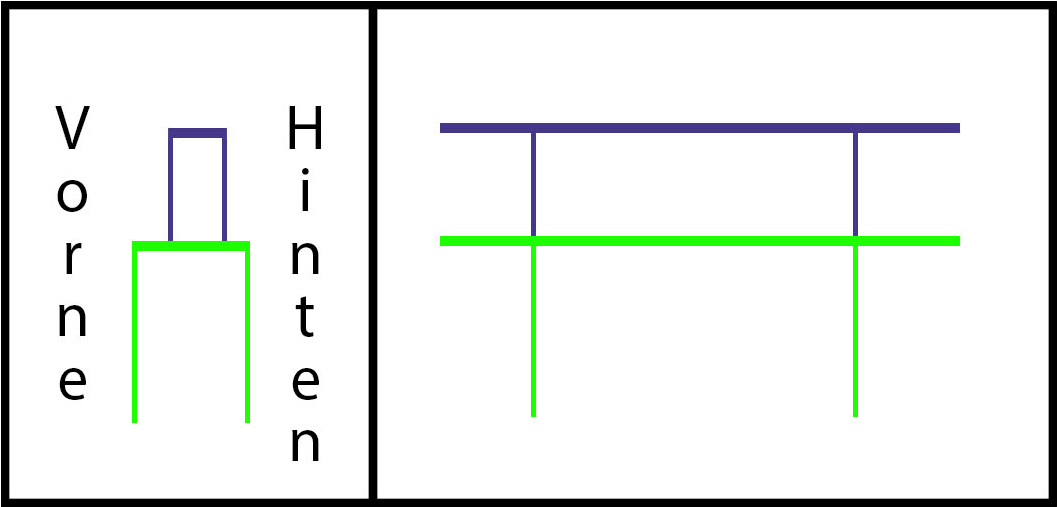
\includegraphics[width=\textwidth]{2d_1.png}
    \caption{Einen Tisch aufstellen und eine aufgeklappte Bank darauf stellen.}
  \end{subfigure}
  \hfill
  \begin{subfigure}[t]{0.45\textwidth}
    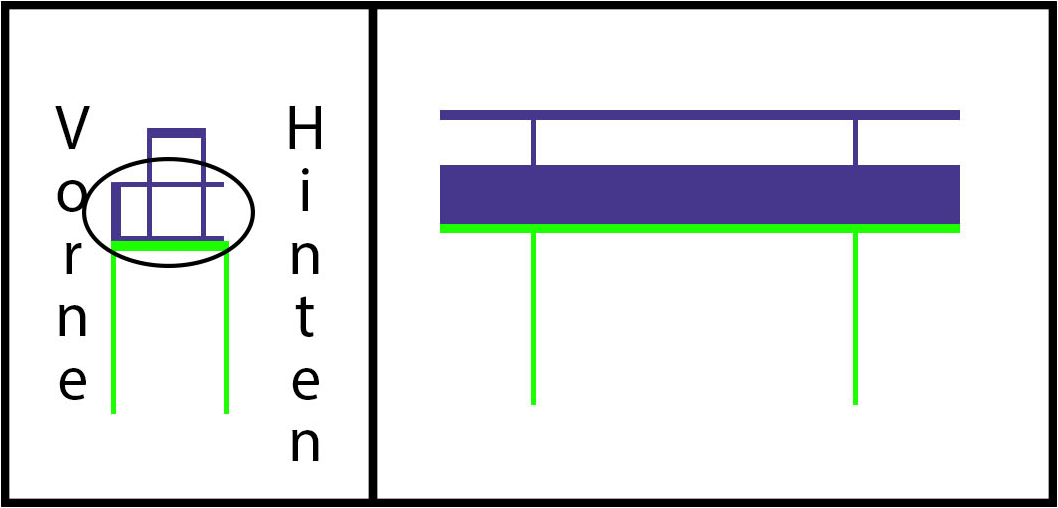
\includegraphics[width=\textwidth]{2d_2.png}
    \caption{Eine Bank aufklappen, aber die diagonalen Arretierungen eingeklappt lassen. Die Bank senkrecht zum Tisch hinlegen und alle drei Teile mit Kabelbindern befestigen, aber noch nicht ganz festzurren.}
  \end{subfigure}
  \centering
  \begin{subfigure}[t]{0.45\textwidth}
    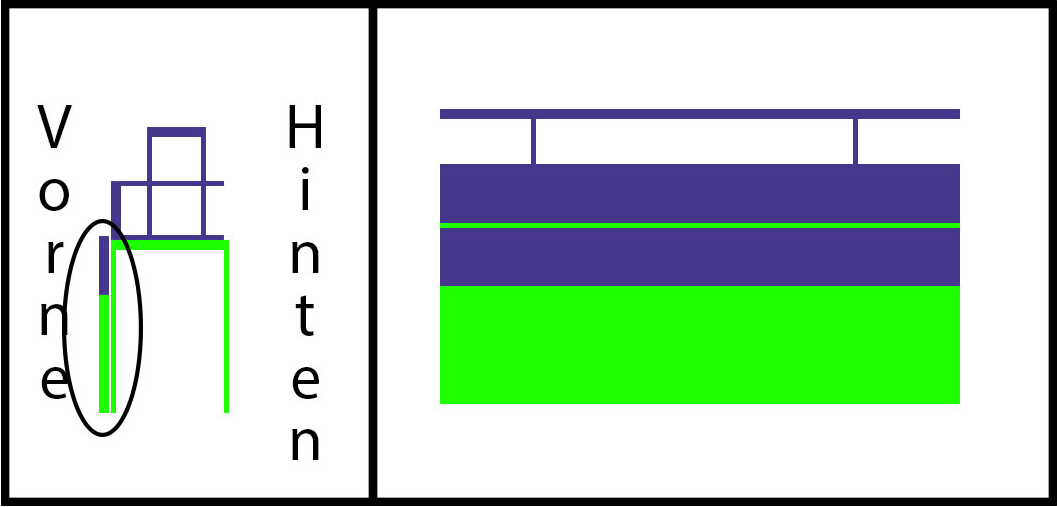
\includegraphics[width=\textwidth]{2d_3.png}
    \caption{Die Vorderseite mit 1 Tisch und 2 Bänken oder 3 Bänken verkleiden und mit Kabelbindern verbinden (die Beine jeweils eingeklappt lassen, sonst stehen sie innen über).}
  \end{subfigure}
  \hfill
  \begin{subfigure}[t]{0.45\textwidth}
    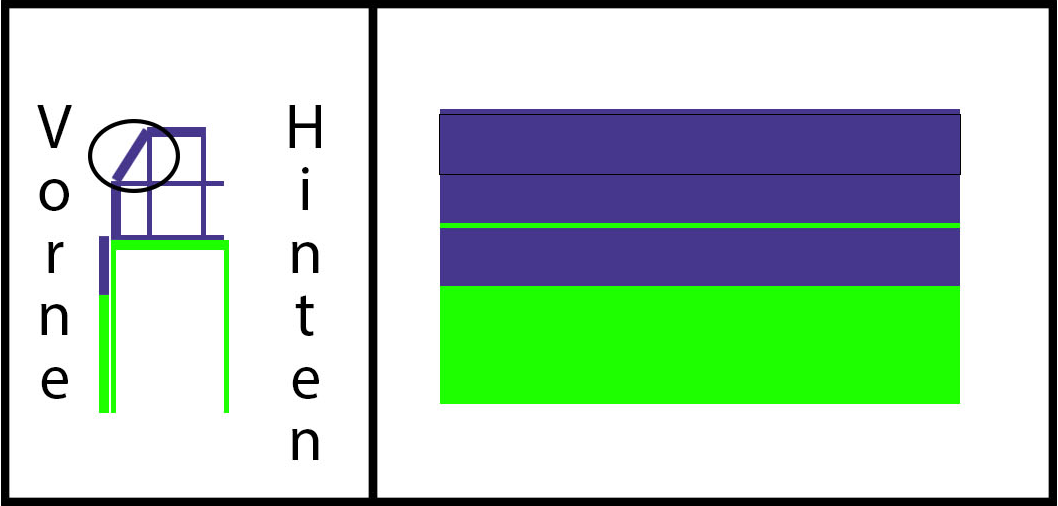
\includegraphics[width=\textwidth]{2d_4.png}
    \caption{Eine Bank (auch ohne Beine) schräg zwischen der liegenden und der stehenden Bank einspannen und mit Kabelbindern festzurren.}
  \end{subfigure}
\end{figure}
% ---
\subsection{Schilder}
\begin{itemize}
  \item Geklebt werden darf auf nur auf unsere Aufbauten und Kühlschränke
  \item Alles nur mit Kreppband Kleben und \textbf{niemals} auf verputzte oder gestrichene Wände!
  \item Aufgehängt werden müssen
    \begin{itemize}
      \item Thekenbeschilderung: Getränkeangebot, laminiert A4/A3 auf die Thekenelemente
      \item Jugendschutzgesetze
    \end{itemize}
  \item Eigene Banner der Fachschaft o.ä.\ müssen mit uns \textbf{rechtzeitig} vorher abgesprochen werden (u.A.\ wegen Brandschutzzertifikat)

    Einfach mitgebrachte Banner können \textbf{nicht} aufgehängt werden!
\end{itemize}
% ---
\subsection{Deadlines}
\begin{itemize}
  \item Zapfanlagen fertig bis \textbf{16:30} für Getränkerundgang und Abnahme der Schankanlagen
  \item Thekenfronten fertig bis \textbf{16:30} für KVR-Rundgang um \textbf{17:00}
  \item Theke innen fertig aufbauen und betriebsfertig machen!

    Alle Getränke zählen und in die angehängte Liste (\emph{Vorher}) eintragen. Nach dem Fest zusammen mit der zweiten ausgefüllten Liste (\emph{Nachher}) einem Getränkeorga geben (Felix, Markus oder Christoph).
  \item \large{Fest beginnt um \textbf{19:00}!}
\end{itemize}
